\doublespacing
\chap{Experiments and Results}


\section{Introduction}

In this chapter, we look at the implementation perspective of the whole system. We also look at the three dataset we used and the results obtained from them. 

\section{Implementation Details}
To implement the conditional generative adversarial network we used Tensorflow\cite{tensorflow2015-whitepaper} with Kera\cite{keras}. The structure of generator and discriminator are described in \cref{Generator-Activation} and \cref{Discriminator-Table}.
\begin{table}[ht]
\centering
\caption{Generator Architecture Specification}
\label{Generator-Activation}
\begin{tabular}{llll}
Operation       & Stride & Features & Activation \\
Merge Input     & -      & -        & -          \\
Dense layer     & -      & -        & Sigmoid    \\
Deconvolution 1 & 5 * 5  & 512      & RELU       \\
Deconvolution 2 & 5 * 5    & 256      & RELU       \\
Deconvolution 3 & 5 * 5   & 128      & RELU       \\
Deconvolution 4 & 5 * 5   & 64       & RELU       \\
Deconvolution 5 & 5 * 5  & 3        & Tanh      
\end{tabular}
\end{table}
\begin{table}[ht]
\centering
\caption{Discriminator Architecture Specification}
\label{Discriminator-Table}
\begin{tabular}{llll}
Operation     & Stride & Features & Activation \\
Convolution 1 & 5 * 5  & 64       & Leaky RELU \\
Convolution 2 & 5*5    & 128      & LeakyRELU  \\
Convolution 3 & 5 *5   & 256      & LeakyRELU  \\
Convolution 4 & 5 *5   & 512      & LeakyRELU  \\
Convolution 5 & 5 * 5  & 1        & Softmax    \\
Convolution 5 & 5*5    & 18       & Sigmoid   
\end{tabular}
\end{table}
\section{Training}
Since the discriminator was weak, before actual training we trained the discriminator in two steps. Firstly we added a conditional vector to its input and removed the classification output of it. And then we trained the discriminator with real images with incorrect label to classify as fake image. Secondly, to the original discriminator we copied the weights from the previous training and trained again on real images to classify the them into the particular class.  
\par

In the below figure we can look at the training losses for the generator and the discriminator. As we can observe after pre-training a GAN, we are able to reach a equilibrium loss for both generator and discriminator at around epoch 30. If we also look at graph closely, in starting epoch the generator and discriminator have a huge loss gap as we are playing minmax game. 

\begin{figure}[H]
  \centering
    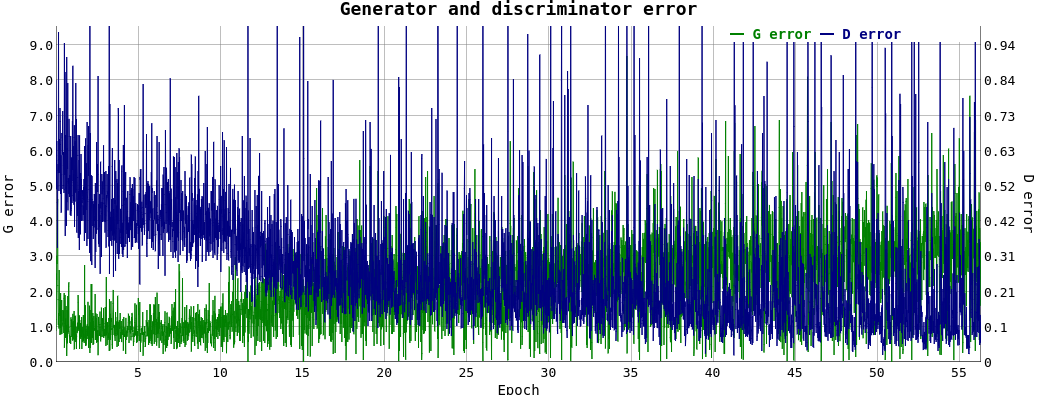
\includegraphics[scale=.4, angle=0]{Files/Training-2.png}
    \caption[Generator Discrminator Loss for Celeba dataset]{}
    \label{fig:train-celeba}
\end{figure}

\begin{figure}[H]
  \centering
    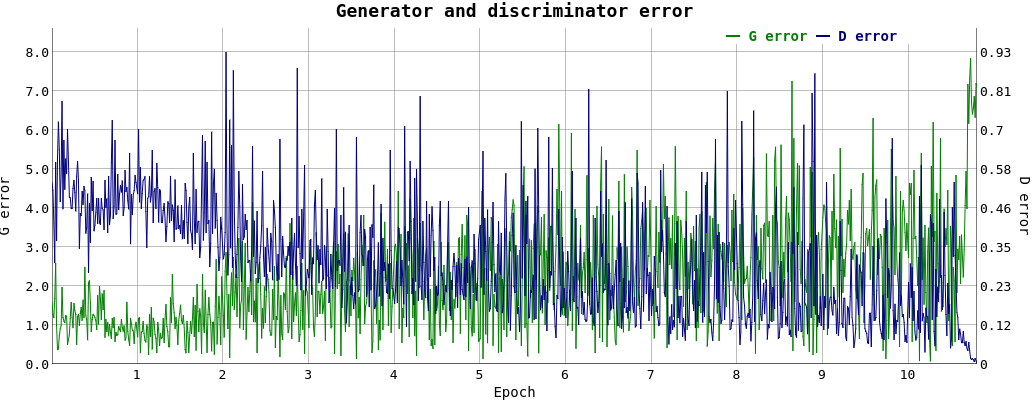
\includegraphics[scale=.4, angle=0]{Files/MNIST-GAN.png}
    \caption[Generator Discrminator Loss for MNIST dataset]{}
    \label{fig:train-mnist}
\end{figure}
\section{DataSet}
\subsection{CelebA}
The CelebFaces Attributes dataset (CelebA)\cite{celeba} contains 202599 face images of celebrities. As some of the categories are very less , so we removed certain categories from our training. . The sdistribution of the overall dataset is shown in \cref{fig:celeba}. As part of preprocessing, we crop the images to $64 \times 64$.The reason for cropping the images is to focus on faces in the images and as they are already aligned.


\begin{figure}[H]
  \centering
    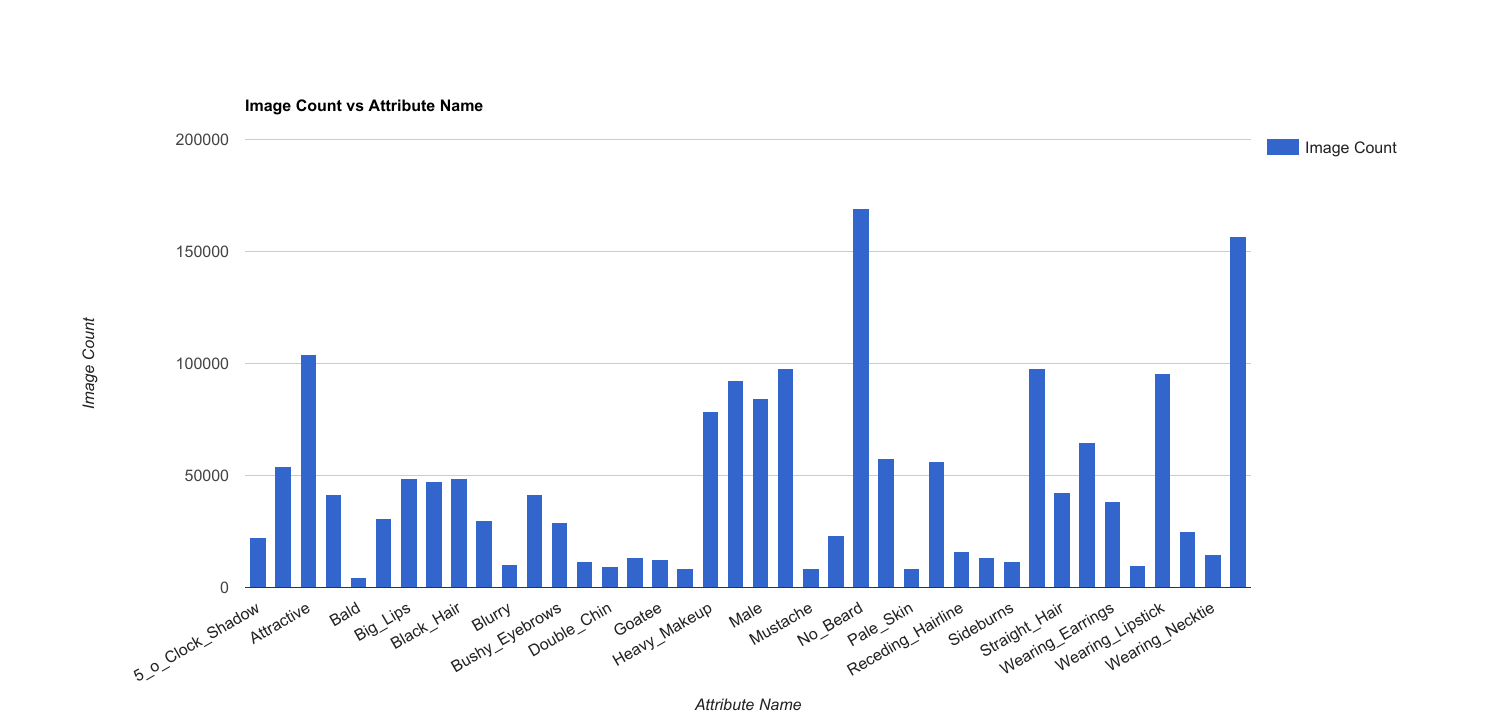
\includegraphics[scale=.3, angle=0]{Files/celeba-visualize.png}
    \caption[Generator Architecture]{Generator Architecture\cite{DCGAN}}
    \label{fig:celeba}
\end{figure}
\subsection{CIFAR-10}

\subsection{MNIST}
The MNIST dataset is very standard image processing dataset. This dataset contains xxx images of digits from 0 to 9. This dataset helps in validating the models correctness in very short time. Since neural  network take lot of time to converge, so if we have some issue with our implementation or logic then we can debug in very short amount of time.

\section{Results}

Once the generator has been trained, we look at the images being generated by our generator. by passing some random noise(z) along with the conditional vector. We can see in \cref{Celeb-a} the various different category facial images being drawn by our generator. There were several categories as shown in \cref{U-celeb-a} for which generator was unsuccessful in getting desired facial attributes.

  

\begin{table}[ht]
\centering
\caption{Successfully Generated Celebrity Images}
\label{Celeb-a}
\begin{tabular}{|llllll|}
\hline
Bald & 
\includegraphics[width=1.69cm, height=1.69cm]{Files/images/images1/image100.png}  &
\includegraphics[width=1.69cm, height=1.69cm]{Files/images/images1/image2.png}   & 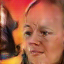
\includegraphics[width=1.69cm, height=1.69cm]{Files/images/images1/image3.png}  & 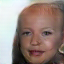
\includegraphics[width=1.69cm, height=1.69cm]{Files/images/images1/image52.png}  & 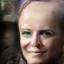
\includegraphics[width=1.69cm, height=1.69cm]{Files/images/images1/image68.png} \\ \hline


Bangs & 
\includegraphics[width=1.69cm, height=1.69cm]{Files/images/images2/image74.png}  &
\includegraphics[width=1.69cm, height=1.69cm]{Files/images/images2/image9.png}   & 
\includegraphics[width=1.69cm, height=1.69cm]{Files/images/images2/image77.png}  & 
\includegraphics[width=1.69cm, height=1.69cm]{Files/images/images2/image79.png}  & 
\includegraphics[width=1.69cm, height=1.69cm]{Files/images/images2/image48.png} \\ \hline


Black Hair & 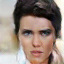
\includegraphics[width=1.69cm, height=1.69cm]{Files/images/images3/image94.png}  &
\includegraphics[width=1.69cm, height=1.69cm]{Files/images/images3/image60.png}   & 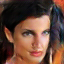
\includegraphics[width=1.69cm, height=1.69cm]{Files/images/images3/image56.png}  & 
\includegraphics[width=1.69cm, height=1.69cm]{Files/images/images3/image87.png}  & 
\includegraphics[width=1.69cm, height=1.69cm]{Files/images/images3/image76.png} \\ \hline


Blond & 
\includegraphics[width=1.69cm, height=1.69cm]{Files/images/images4/image86.png}  &
\includegraphics[width=1.69cm, height=1.69cm]{Files/images/images4/image64.png}   & 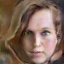
\includegraphics[width=1.69cm, height=1.69cm]{Files/images/images4/image91.png}  & 
\includegraphics[width=1.69cm, height=1.69cm]{Files/images/images4/image5.png}  & 
\includegraphics[width=1.69cm, height=1.69cm]{Files/images/images4/image25.png} \\ \hline


Male & 
\includegraphics[width=1.69cm, height=1.69cm]{Files/images/images10/image12.png}  &
\includegraphics[width=1.69cm, height=1.69cm]{Files/images/images10/image32.png}   & 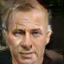
\includegraphics[width=1.69cm, height=1.69cm]{Files/images/images10/image19.png}  & 
\includegraphics[width=1.69cm, height=1.69cm]{Files/images/images10/image34.png}  & 
\includegraphics[width=1.69cm, height=1.69cm]{Files/images/images10/image55.png} \\ \hline

Mouth Open  & 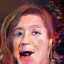
\includegraphics[width=1.69cm, height=1.69cm]{Files/images/images11/image70.png}  &
\includegraphics[width=1.69cm, height=1.69cm]{Files/images/images11/image69.png}   & 
\includegraphics[width=1.69cm, height=1.69cm]{Files/images/images11/image65.png}  & 
\includegraphics[width=1.69cm, height=1.69cm]{Files/images/images11/image37.png}  & 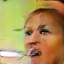
\includegraphics[width=1.69cm, height=1.69cm]{Files/images/images11/image7.png} \\ \hline

Smiling  & 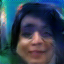
\includegraphics[width=1.69cm, height=1.69cm]{Files/images/images15/image70.png}  &
\includegraphics[width=1.69cm, height=1.69cm]{Files/images/images15/image7.png}   & 
\includegraphics[width=1.69cm, height=1.69cm]{Files/images/images15/image47.png}  & 
\includegraphics[width=1.69cm, height=1.69cm]{Files/images/images15/image37.png}  & 
\includegraphics[width=1.69cm, height=1.69cm]{Files/images/images15/image76.png} \\ \hline

Eye Glasses  & 
\includegraphics[width=1.69cm, height=1.69cm]{Files/images/images7/image79.png}  &
\includegraphics[width=1.69cm, height=1.69cm]{Files/images/images7/image4.png}   & 
\includegraphics[width=1.69cm, height=1.69cm]{Files/images/images7/image27.png}  & 
\includegraphics[width=1.69cm, height=1.69cm]{Files/images/images7/image25.png}  & 
\includegraphics[width=1.69cm, height=1.69cm]{Files/images/images7/image67.png} \\ \hline

Eye Glasses  & 
\includegraphics[width=1.69cm, height=1.69cm]{Files/images/images7/image79.png}  &
\includegraphics[width=1.69cm, height=1.69cm]{Files/images/images7/image4.png}   & 
\includegraphics[width=1.69cm, height=1.69cm]{Files/images/images7/image27.png}  & 
\includegraphics[width=1.69cm, height=1.69cm]{Files/images/images7/image25.png}  & 
\includegraphics[width=1.69cm, height=1.69cm]{Files/images/images7/image67.png} \\ \hline
\end{tabular}
\end{table}

\begin{table}[H]
\centering
\caption{Unsuccessful Generated Celebrity Images}
\label{U-celeb-a}
\begin{tabular}{|llllll|}
\hline
Wearing Hat & 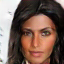
\includegraphics[width=1.69cm, height=1.69cm]{Files/images/images18/image1.png}  &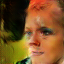
\includegraphics[width=1.69cm, height=1.69cm]{Files/images/images18/image2.png}   & \includegraphics[width=1.69cm, height=1.69cm]{Files/images/images18/image3.png}  & \includegraphics[width=1.69cm, height=1.69cm]{Files/images/images18/image52.png}  & \includegraphics[width=1.69cm, height=1.69cm]{Files/images/images18/image68.png} \\ \hline


Wavy Hair & \includegraphics[width=1.69cm, height=1.69cm]{Files/images/images17/image1.png}  &\includegraphics[width=1.69cm, height=1.69cm]{Files/images/images17/image2.png}   & \includegraphics[width=1.69cm, height=1.69cm]{Files/images/images17/image3.png}  & \includegraphics[width=1.69cm, height=1.69cm]{Files/images/images17/image52.png}  & \includegraphics[width=1.69cm, height=1.69cm]{Files/images/images17/image68.png} \\ \hline

Receding Hairline & \includegraphics[width=1.69cm, height=1.69cm]{Files/images/images14/image1.png}  &\includegraphics[width=1.69cm, height=1.69cm]{Files/images/images14/image2.png}   & \includegraphics[width=1.69cm, height=1.69cm]{Files/images/images14/image3.png}  & \includegraphics[width=1.69cm, height=1.69cm]{Files/images/images14/image52.png}  & \includegraphics[width=1.69cm, height=1.69cm]{Files/images/images14/image68.png} \\ \hline


\end{tabular}
\end{table}

\begin{table}[ht]
\centering
\caption{Successfully Generated MNIST Images}
\label{MNIST-Result}
\begin{tabular}{|llllll|}
\hline
0 & \includegraphics[width=1.69cm, height=1.69cm]{Files/MNIST/9.9915 [www.imagesplitter.net]-0-0.png}  &\includegraphics[width=1.69cm, height=1.69cm]{Files/MNIST/9.9915 [www.imagesplitter.net]-1-2.png}   & \includegraphics[width=1.69cm, height=1.69cm]{Files/MNIST/9.9915 [www.imagesplitter.net]-2-4.png}  & \includegraphics[width=1.69cm, height=1.69cm]{Files/MNIST/9.9915 [www.imagesplitter.net]-5-0.png}  & \includegraphics[width=1.69cm, height=1.69cm]{Files/MNIST/9.9915 [www.imagesplitter.net]-6-2.png} \\ \hline
\end{tabular}
\end{table}



\section{Evaluation}

It is very challenging to evaluate the performance of GAN networks as there has been no comparable method to judge the quality of images being produced. So, to evaluate and examine the performance we devised two methods. In the first method we will use the same discriminator to evaluate the accuracy of these images. The \cref{} shows the overall accuracy of the images of different dataset when passed through same discriminator.  


Also to examine the over-fitting we look at the latent space. 